\documentclass[11pt,english]{article}

\usepackage[english]{babel}
\usepackage{enumitem}
\usepackage{fancyhdr}
\usepackage{graphicx}
\usepackage{lastpage}

\pagestyle{fancy}

\graphicspath{{assets/}}

\lfoot{}
\cfoot{\today}
\rfoot{\thepage/\pageref{LastPage}}

\newcommand*{\Frontpage}{\begingroup
  \hbox{%
    \hspace*{0.2\textwidth}
    \rule{1pt}{\textheight}
    \hspace*{0.05\textwidth}
    \parbox[b]{0.75\textwidth}{%
      {\noindent\Huge\bfseries IDPRI}\\[2\baselineskip] % Title
      {\large \textit{Huiswerkopdrachten}}\\[4\baselineskip] % Tagline or further description
      {\Large \textsc{\\
          Patrick Spek, 2099745 \\
          Roy, 2097591 \\
        }}
      \vspace{0.5\textheight} % Whitespace between the title block and the publisher
    }
  }
\endgroup}

\renewcommand{\footrulewidth}{0.4pt}

\begin{document}
  \thispagestyle{empty}
  \Frontpage
  \newpage

  \tableofcontents
  \newpage

  \section{Opdracht 1}
  \subsection{Goede designs}
  \subsubsection{Website}
  \begin{center}
    \makebox[\textwidth]{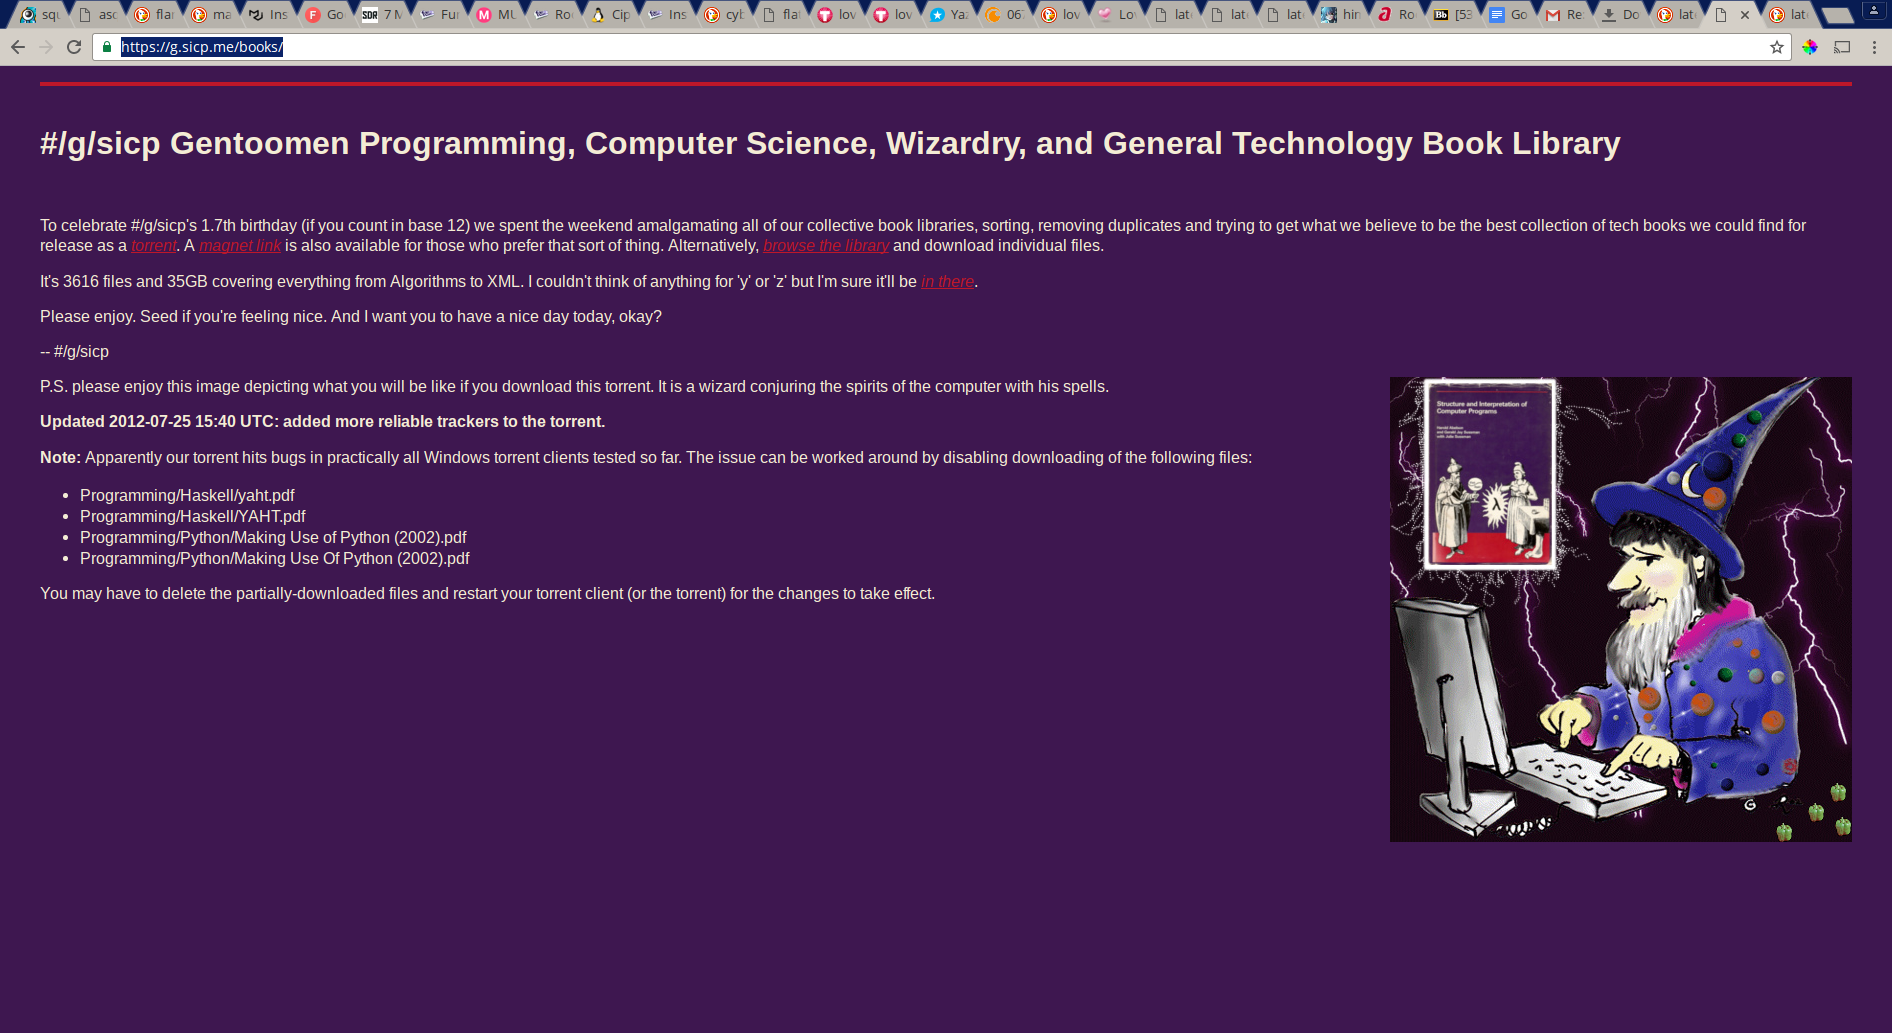
\includegraphics[width=\linewidth]{website-goed}}
  \end{center}
  Website is snel, duidelijk en werkt op alle browsers ooit.
  
  \subsubsection{Game}
  \begin{center}
    \makebox[\textwidth]{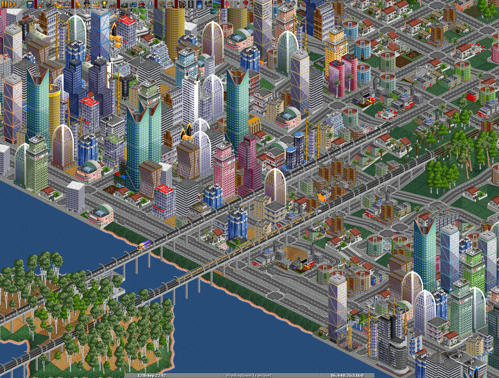
\includegraphics[width=\linewidth]{game-goed}}
  \end{center}
  OpenTTD is een kleine applicatie die op elk OS werkt.
  
  \subsubsection{App}

  \subsubsection{Gebruiksvoorwerp}
  \begin{center}
    \makebox[\textwidth]{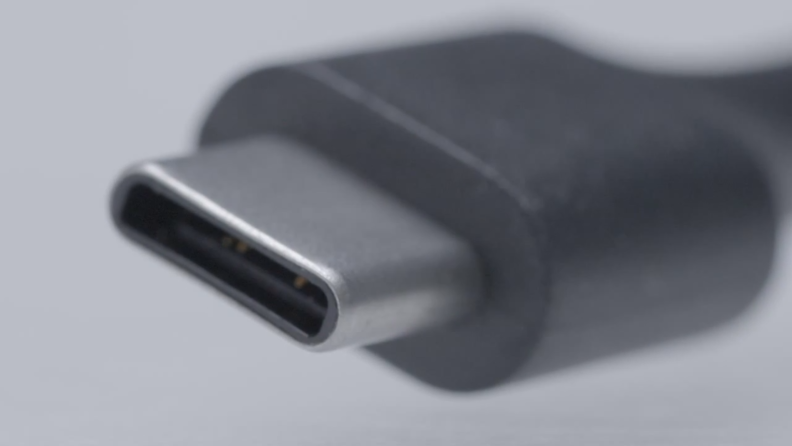
\includegraphics[width=\linewidth]{voorwerp-goed}}
  \end{center}
  USB Type C is een verbetering ten opzichte van A en B omdat deze altijd in de
  goede positie zit.

  \subsection{Slechte designs}
  \subsubsection{Website}
  \begin{center}
    \makebox[\textwidth]{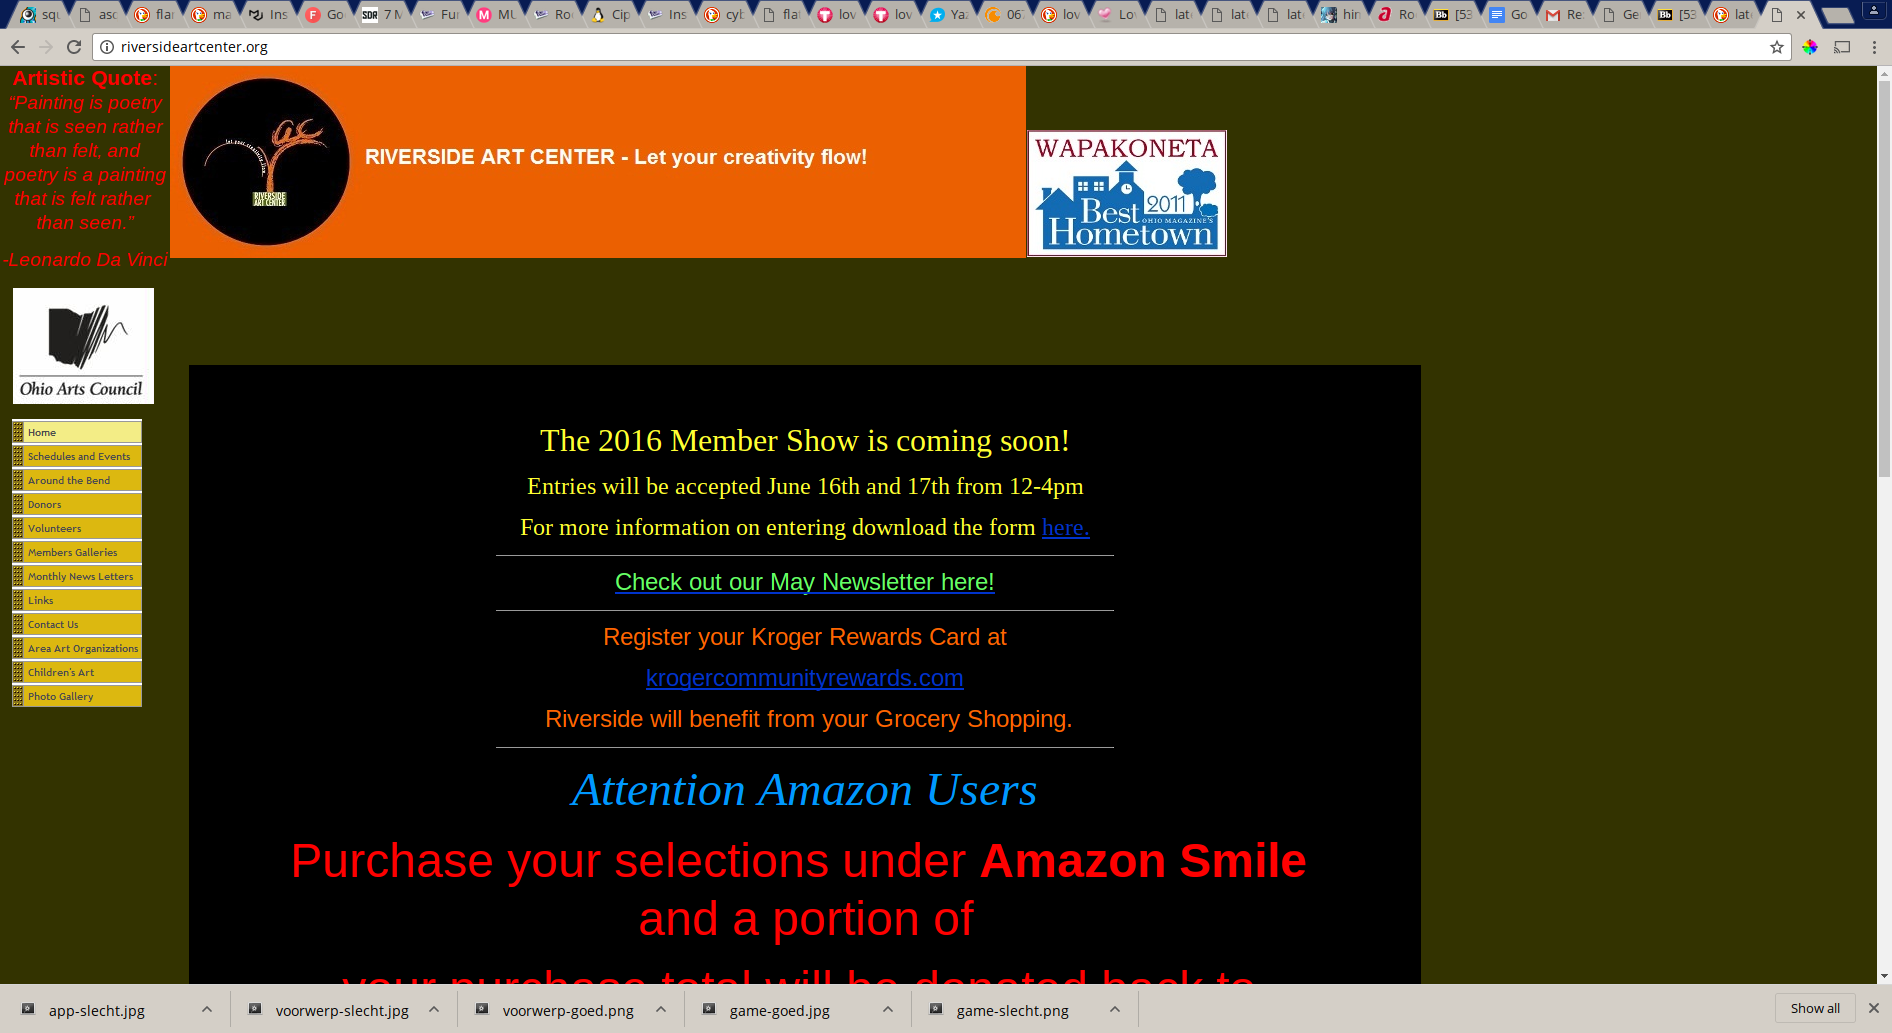
\includegraphics[width=\linewidth]{website-slecht}}
  \end{center}
  Fonts zijn lelijk, kleuren zijn nog lelijker.

  \subsubsection{Game}
  \begin{center}
    \makebox[\textwidth]{
\includegraphics[width=\linewidth]{game-slecht}}
  \end{center}
  Game runt poep.

  \subsubsection{App}
  \begin{center}
    \makebox[\textwidth]{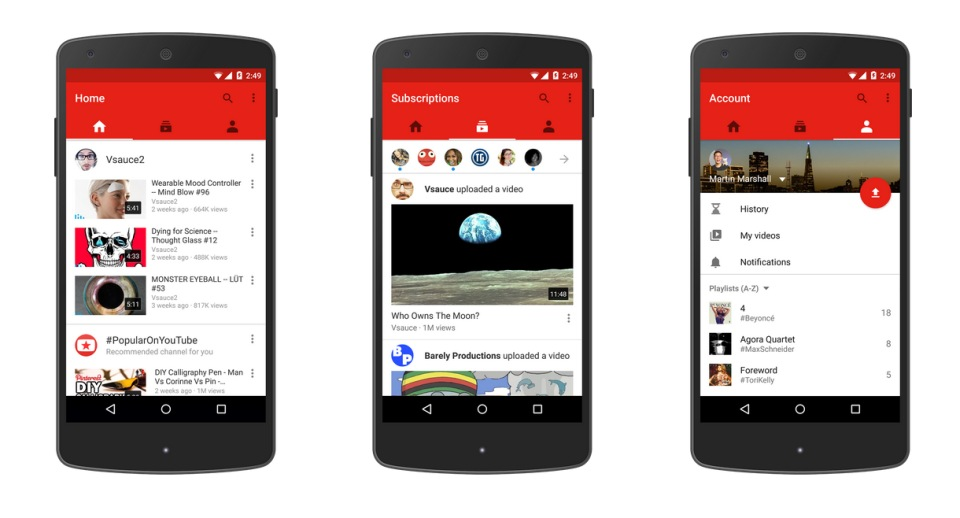
\includegraphics[width=\linewidth]{app-slecht}}
  \end{center}
  De YouTube app speelt geen videos door wanneer de app niet in de voorgrond is.
  Dit is kut.

  \subsubsection{Gebruiksvoorwerp}
  \begin{center}
    \makebox[\textwidth]{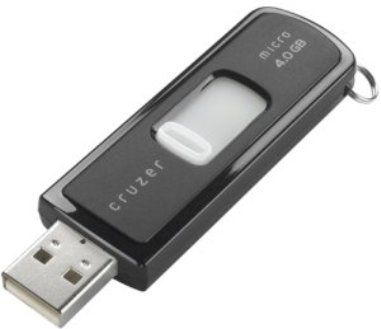
\includegraphics[width=\linewidth]{voorwerp-slecht}}
  \end{center}
  USB Type A is (vergeleken met Type C) niet gebruiksvriendelijk (tenzij je weet
  hoe zo'n ding werkt).

  \newpage
  \section{Opdracht 3}
  \begin{itemize}
    \item \textbf{Het aanmaken van issues} \\
      Een BTS is zinloos als je geen issues kunt aanmaken.
    \item \textbf{Het aangeven van prioriteiten bij issues} \\
      Hiermee kan een developer direct zien welke issues belangrijker zijn om te
      fixen voor de volgende release.
    \item \textbf{Parent/child issue relaties} \\
      Hiermee kan de developer zien welke issues moeten worden opgelost voordat
      andere issues opgelost kunnen worden.
    \item \textbf{Milestone voor issues} \\
      Hiermee kun je feature-issues aan een release linken, zodat je een
      makkelijk overzicht kunt maken om de taken voor een volgende release in te zien.
    \item \textbf{Comments} \\
      Met comments kun je feedback vragen van andere developers of meer
      informatie vragen van de reported als de issue origineel niet duidelijk is.
  \end{itemize}
\end{document}

